
\subsection{Ejercicios}
\begin{itemize}
 \item 
\textbf{Ejercicio 3}  Completar la implementacion del scheduler Round-Robin implementando los
metodos de la clase SchedRR en los archivos sched rr.cpp y sched rr.h. La implementacion
recibe como primer parametro la cantidad de nucleos y a continuacion los valores de sus
respectivos quantums. Debe utilizar una unica cola global, permitiendo ası la migracion de
procesos entre nucleos.
\item \textbf{Ejercicio 4} Diseñar uno o mas lotes de tareas para ejecutar con el algoritmo del ejercicio
anterior. Graficar las simulaciones y comentarlas, justificando brevemente por que el comportamiento 
observado es efectivamente el esperable de un algoritmo Round-Robin.
\item \textbf{Ejercicio 5} A partir del artıculo
Waldspurger, C.A. and Weihl, W.E., Lottery scheduling: Flexible proportional-share re-
source management. Proceedings of the 1st USENIX conference on Operating Systems
Design and Implementation – 1994.
diseñar e implementar un scheduler basado en el esquema de loterıa. El constructor de la
clase SchedLottery debe recibir dos parametros: el quantum y la semilla de la secuencia
pseudoaleatoria (en ese orden). Interesa implementar al menos la idea basica del algoritmo
y la optimizacion de tickets compensatorios (compensation tickets). Otras optimizaciones y
refinamientos que propone el artıculo seran opcionales siempre que, en cada caso, se explique
brevemente por que la optimizacion no se considero relevante a los efectos de este trabajo.

\end{itemize}


\subsection{Resultados y Conclusiones}

\subsubsection[Resolución Ejercicio 3]{Ejercicio 3}

\indent \indent Para completar la implementación del scheduler Round-Robin y que su comportamiento sea correcto, hicimos uso de diversas estructuras de datos cuya composición y uso describimos a continuación.\\
\begin{itemize}
\item Una cola global FIFO nombrada $q$, que contiene los pid de las tareas activas no bloqueadas y cuyo tope representa a la próxima tarea a correr. 
Utilizando una cola FIFO podemos obtener el comportamiento deseado, ya  que al desalojarse una tarea por consumir su quantum esta misma será agregada nuevamente a la cola, quedando al final de ésta y generando el ciclo que buscamos.
Al ser además la única cola para todos los cores, no se restringe a una tarea a ser ejecutada por un único núcleo, permitiendo así la migración entre nucleos.\\
\item El vector $cores$ contiene en su elemento $i$ y el pid correspondiente a la tarea que está corriendo en el core $i+1$. Inicializamos todos sus elementos en $-1$ (que se corresponde con la Idle Task) para reconocer que no se han cargado tareas en los núcleos de procesamiento.\\
\item De la misma manera, el vector $quantum$ contiene en la posición $i$ el quantum definido para el núcleo y el vector $quantumActual$, contiene la cantidad de ticks que le quedan desde que se cargó la tarea en el core. 
En conjunto, ambas estructuras nos permiten determinar cuándo se consumió el quantum de una tarea, de manera tal que podamos desalojarla.\\
\end{itemize}
\indent Ademas, tomamos ciertas decisiones en esta implementación las cuales detallamos a continuacion:
\begin{itemize}
 \item Si una tarea se encuentra bloqueada cuando se produce el tick del reloj, esta misma es desalojada de la cola global, 
 y agregada en un lista de $bloqueados$. A su vez, será reseteado el quantum, se le dara inicio a la proxima tarea que se encuentre
 ready y cuando el sistema operativo, nos envie una señal de unblock, la tarea desalojada regresara al final de la cola global.
\end{itemize}


\subsubsection[Resolución Ejercicio 4]{Ejercicio 4}

\indent El algoritmo de scheduling Round-Robin se basa en asignar a las tareas un tiempo determinado de procesamiento en porciones equitativas  con un orden cíclico, llamado
$quantum$. 
Esto se hace definiendo para cada núcleo de procesamiento un valor de $quantum$ y cada tarea que corre en ese núcleo lo hará a lo sumo por un tiempo igual a éste. 
Si la tarea consume su quantum pero no terminó su ejecución, se la envia a la cola global y se asigna el procesador a la siguiente tarea, en 
caso de que hubiese, que correrá a lo sumo por la cantidad de $quantum$ indicada. 
Una vez que todas las tareas corrieron, se vuelve a asignar tiempo de procesamiento a la primera tarea, 
de ahí el comportamiento ciclico circular del algoritmo.\\
\indent A su vez, puede ocurrir que una tarea no consuma todo su $quantum$. Ya sea porque 
la tarea terminó su ejecución o bien se bloqueó haciendo uso de entrada/salida.\\
\indent En caso de haber terminado, el algoritmo se pone a correr la tarea siguiente de acuerdo al orden circular que se 
establecio y la tarea que terminó se desalojara por completo y no sera nuevamente considerada.\\
\indent En caso que se haya bloqueado, esta mimsa dejará de ser considerada hasta que se desbloquee. Mientras tanto,
seguiran corriendo las demas tareas que no esten bloqueadas respetando el orden ciclico.
Cuando esta tarea se desbloquee puede no respetar el orden que se habia establecido. Por ej. en nuestra implementacion
si la tarea esta bloqueada al recibir un tick, esta misma se la quita de la ejecucion y una ves desbloqueada pasara al final de
la cola global.\\

\indent Para poder verificar si el comportamiento era el deseado de nuestra implementación del algoritmo en cuestión, 
desarrollamos 3 diversos lotes de tareas ($taskCPU$ y $taskConsola$), los cuales fueron chequeados con 1,2 y 3 cores.\\
Trabajando con los mismos $quantum$ cada core.
\indent

Nuestro primer lote de tareas fue el siguiente:
\begin{verbatim}
                                     TaskCPU 70
                                     TaskConsola 2 4 5
                                     TaskCPU 40
                                     TaskConsola 3 2 3
                                     TaskCPU 30
\end{verbatim}

Utilizando este lote, obtuvimos los siguientes gráficos de simulación:\\
\begin{center}

    
	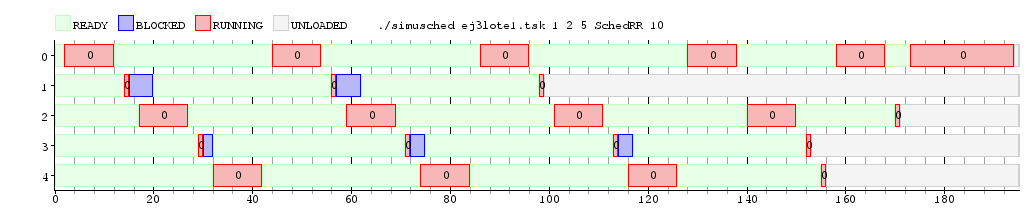
\includegraphics[width=450pt]{./EJ4_RR/ejercicio4-1nucleo.png}
	{$Lote 1$ - Scheduler RR - 1 core}	
 
\end{center}


\indent Con esta simulación, trabajamos con 2 ticks de cambio de contexto y 5 de cambio de procesador, el cual no presta importancia
en la simulación trabajando con un core.\\
\\
\indent Se puede observar el cambio de tareas cíclico tanto porque terminaron su quantum o porque se bloquearon.\\

\begin{center}
  	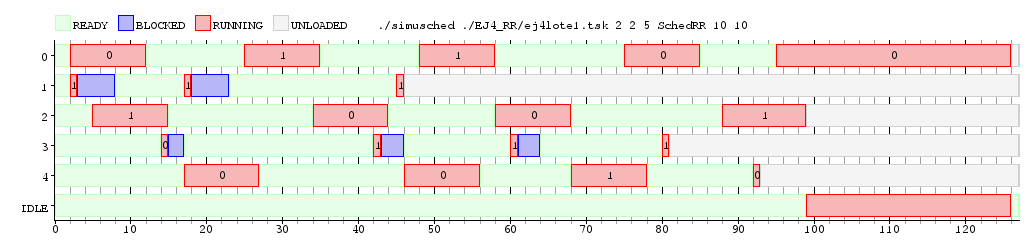
\includegraphics[width=450pt]{./EJ4_RR/ejercicio4-2nucleo.png}
	  {$Lote 1$ - Scheduler RR - 2 core}	
\end{center}

\begin{center}
  	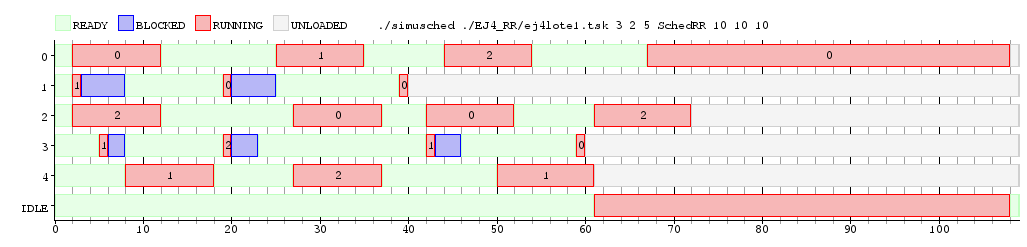
\includegraphics[width=450pt]{./EJ4_RR/ejercicio4-3nucleo.png}
	  {$Lote 1$ - Scheduler RR - 3 core}	
\end{center}

\indent Se ha podido notar, ademas del la ejecucion circular de las tareas, un cierto paralelismo al estar trabajando con
2 o 3 cores.\\

\indent Luego, de esta simulación probamos con un lote con tareas que se bloqueen por más tiempo:
 \begin{verbatim}
                                     TaskCPU 70
                                     TaskConsola 5 6 7
                                     TaskCPU 40
                                     TaskConsola 10 9 8
                                     TaskCPU 30
 \end{verbatim}

\indent Manteniendo la misma cantidad de tick para cambio de contexto y core. Y manteniendo los mismos valores
de $quantum$ obtuvimos los siguientes gráficos:

\begin{center}
    	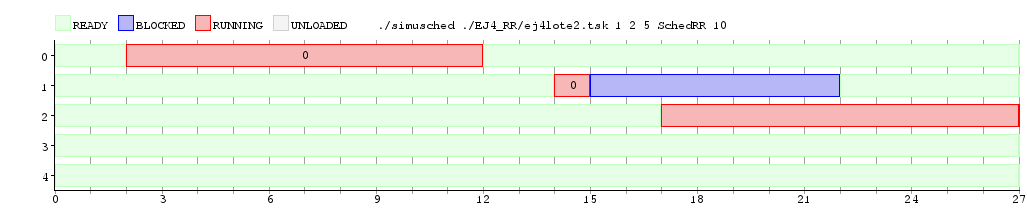
\includegraphics[width=450pt]{./EJ4_RR/ejercicio4-2lote1nucleo.png}
	{$Lote 2$ - Scheduler RR - 1 core}	
 \end{center}

 \begin{center}
    	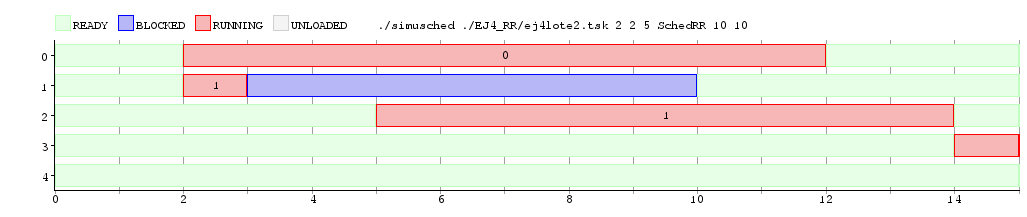
\includegraphics[width=450pt]{./EJ4_RR/ejercicio4-2lote2nucleo.png}
	{$Lote 2$ - Scheduler RR - 2 core}	
 \end{center}
 
 \begin{center}
    	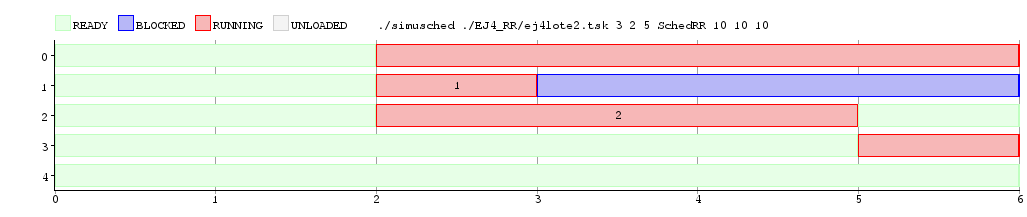
\includegraphics[width=450pt]{./EJ4_RR/ejercicio4-2lote3nucleo.png}
	{$Lote 2$ - Scheduler RR - 3 core}	
 \end{center}

 \indent Con este lote, además de lo observado anteriormente pudimos ver que, al tener una tarea bloqueada
 por un largo tiempo, el scheduler directamente la ignora.\\
 
\indent Luego de los gráficos pudimos observar lo siguiente sobre el comportamiento del Round-Robin:\\
\begin{itemize}
\item  Carácter circular del algoritmo.
\item  Desalojo de las tareas cuando se bloquean o terminan y la inmediata asignación del núcleo a la siguiente tarea en caso de existir alguna.
\item  Libre de inanición.
\item  Una tarea bloqueada es ignorada por el scheduler hasta que se desbloquee.
\end{itemize}

\indent Finalmente, dado su carácter circular y equitativo, podemos afirmar que todas las tareas que 
estén en condiciones de correr serán ejecutadas y ninguna será negada de tiempo de procesamiento.\\

\subsubsection[Resolución Ejercicio 5]{Ejercicio 5}

\begin{center}
\textbf{Lottery Scheduling} 
\end{center}

\indent Lottery Scheduling se trata de un mecanismo que asigna recursos de manera aleatoria. Dando lugar a que cada proceso
tenga una probabilidad p de ejecutarse. \\
Esta probabilidad de ganar un recurso, está representada por billetes de lotería (o tickets). A la hora de asignar un recurso
(procesador) a un proceso se celebra una lotería, en la que un recurso es asignado al proceso con el ticket ganador.\\
Esto permite asignar los recursos eficaz y proporcionalmente.\\

\begin{center}
\textbf{Implementación de la idea básica del algoritmo} 
\end{center}

\indent Para llevar a cabo este concepto, se implementó la idea de asignación de tickets por proceso. 
Es decir, que a cada proceso nuevo que llegue, el scheduler le asigna una cantidad determinada de tickets. \\
Esta cantidad de tickets en principio es igual para todos los procesos.\\
Por eso a la hora de cargarse un nuevo proceso, se recalcula la cantidad total de tickets.\\

\indent El cálculo de la cantidad total de tickets y de los tickets que le corresponden a un proceso nuevo es el siguiente:\\
\begin{itemize}
 \item tickets\_totales = QUANTUM $*$ cantidad\_de\_procesos $*$ 1000;
 \item tickets\_de\_un\_proceso = tickets\_totales/cantidad\_de\_procesos;
\end{itemize}

\indent Luego de esta asignación de tickets, la idea del algoritmo es sencilla. \\
Se elige un ticket ganador mediante la función rand entre 0 y la cantidad total de tickets menos uno. Para esto, previamente ya habíamos configurado (al construirse el scheduler) la semilla del
generador de numeros aleatorios pasada por parámetro con la función srand.\\
Una vez conseguido el ticket ganador, hay un proceso ganador del quantum, y debemos buscarlo en la lista de procesos. \\
El quantum es un parámetro que usamos para que el proceso pueda correr más de un tick de reloj. 
El proceso ganador puede no llegar a terminar su quantum, ya que se bloqueó. \\
En caso de bloquearse el proceso, se lo saca de la lista de procesos disponibles, 
para que el scheduler no lo tenga en cuenta hasta que el mismo se desbloquee. \\
Al desbloquearse, el scheduler simplemente lo agrega de nuevo a la lista de procesos disponibles con la misma cantidad de
tickets de un proceso nuevo.\\\\

Entonces, se puede afirmar, que todos los procesos tienen la misma probabilidad de ser elegidos por el scheduler.\\

\begin{center}
 \textbf{Optimización de tickets compensatorios}
\end{center}

La idea de esta opimización es sencilla. Se trata de darle más probabilidad de ganar el quantum al proceso que fue bloqueado.
Cuando un proceso se bloquea, no terminó todo el quantum que había ganado.\\
Sabiendo esto, guardamos el pid del proceso a bloquearse en una lista de bloqueados, y también guardamos en otra lista 
el quantum que consumió.\\
Al desbloquearse, en vez de agregarlo una vez a la lista de procesos disponibles, lo agregamos la cantidad de veces como ticks 
le faltaba para terminar el quantum antes de bloquearse. \\
Por ejemplo, si el quantum es de 10 y consumió solo 4, lo agregamos 4 veces a la lista de procesos. 
Y aca está el punto clave de la optimización: el proceso bloqueado en realidad tiene más tickets que un proceso 
que no se bloqueó, en el ejemplo, 4 veces más. Por lo tanto tiene más posibilidades de volver a ser elegido.\\